\newcommand{\figureDigitalSignalExample}[1]{
  \begin{figure}[ht]
    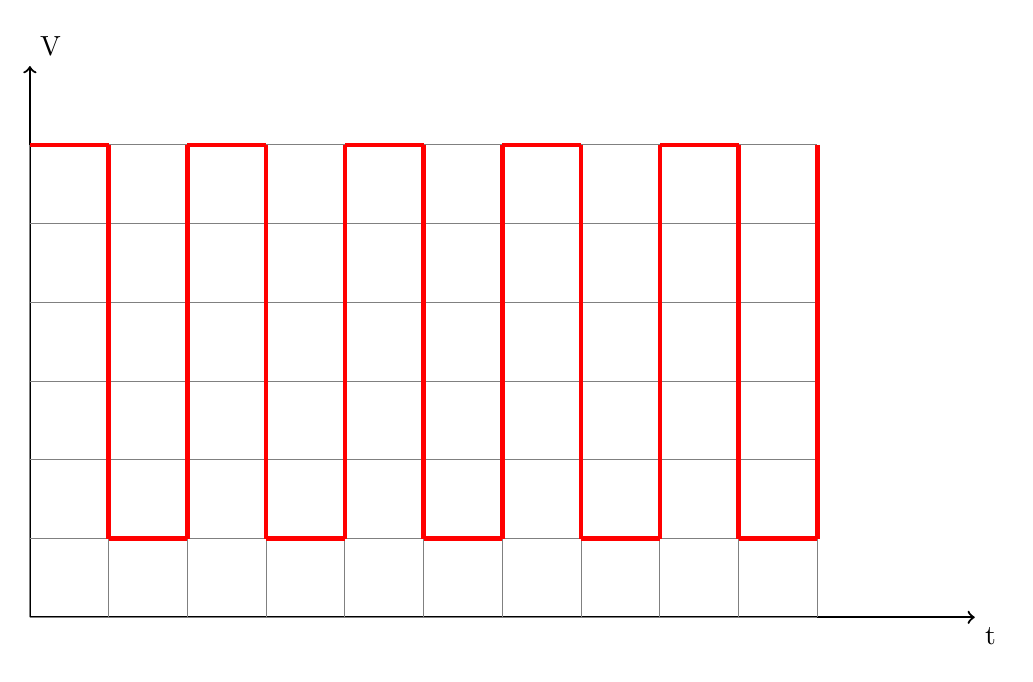
\begin{tikzpicture}
      \draw[thick, ->] (0, 0) -- (12, 0) node[anchor=north west] {t};
      \draw[thick, ->] (0, 0) -- (0,  7) node[anchor=south west] {V};
      \draw[gray] (0, 0) grid (10, 6);
      \foreach \x in {0, 2, ..., 8} {
        \draw[ultra thick, red] (\x, 6) -- (\x + 1, 6);
        \draw[ultra thick, red] (\x + 1, 6) -- (\x + 1, 1);
        \draw[ultra thick, red] (\x + 1, 1) -- (\x + 2, 1);
        \draw[ultra thick, red] (\x + 2, 1) -- (\x + 2, 6);
      }
    \end{tikzpicture}
    \caption{#1}
    \label{fig:adc-digital-signal-example}
  \end{figure}
}
